\documentclass[12pt, block=fill]{beamer}
\usepackage[sfdefault]{FiraSans}
\usepackage{FiraMono}
\usepackage[T1]{fontenc}
\usepackage{xcolor}

\usepackage{pgfpages}
\setbeameroption{hide notes} % Only slides
% \setbeameroption{show only notes} % Only notes
 % \setbeameroption{show notes on second screen=right} % Both

\definecolor{burntOrange}{rgb}{.8, .5, .1}
\definecolor{textgray}{rgb}{.8,.8,.8}

\usetheme[titleformat frame = smallcaps]{metropolis}

\metroset{block=fill}

\newcommand{\E}{\text{E}}
\newcommand{\V}{\text{V}}
\newcommand{\cov}{\text{cov}}

\begin{document}

%Section 7.06 Edits start

\section{The Independent Samples t-Test}

\begin{frame}
  \frametitle{Comparing Population Means}
  \begin{exampleblock}{t-Test}
    Tells us whether the means of two sample populations are significantly different from each other 
  \end{exampleblock}

  For example:
  \begin{itemize}
      \item Suppose we have two groups
      \begin{itemize}
          \item Stanford students
          \item Berkeley students
      \end{itemize}
      \item We want to compare the average attractiveness of these two groups to see if one group is significantly more attractive
  \end{itemize}
\end{frame}

\begin{frame}
  \frametitle{Comparing Population Means}
    \begin{center}
        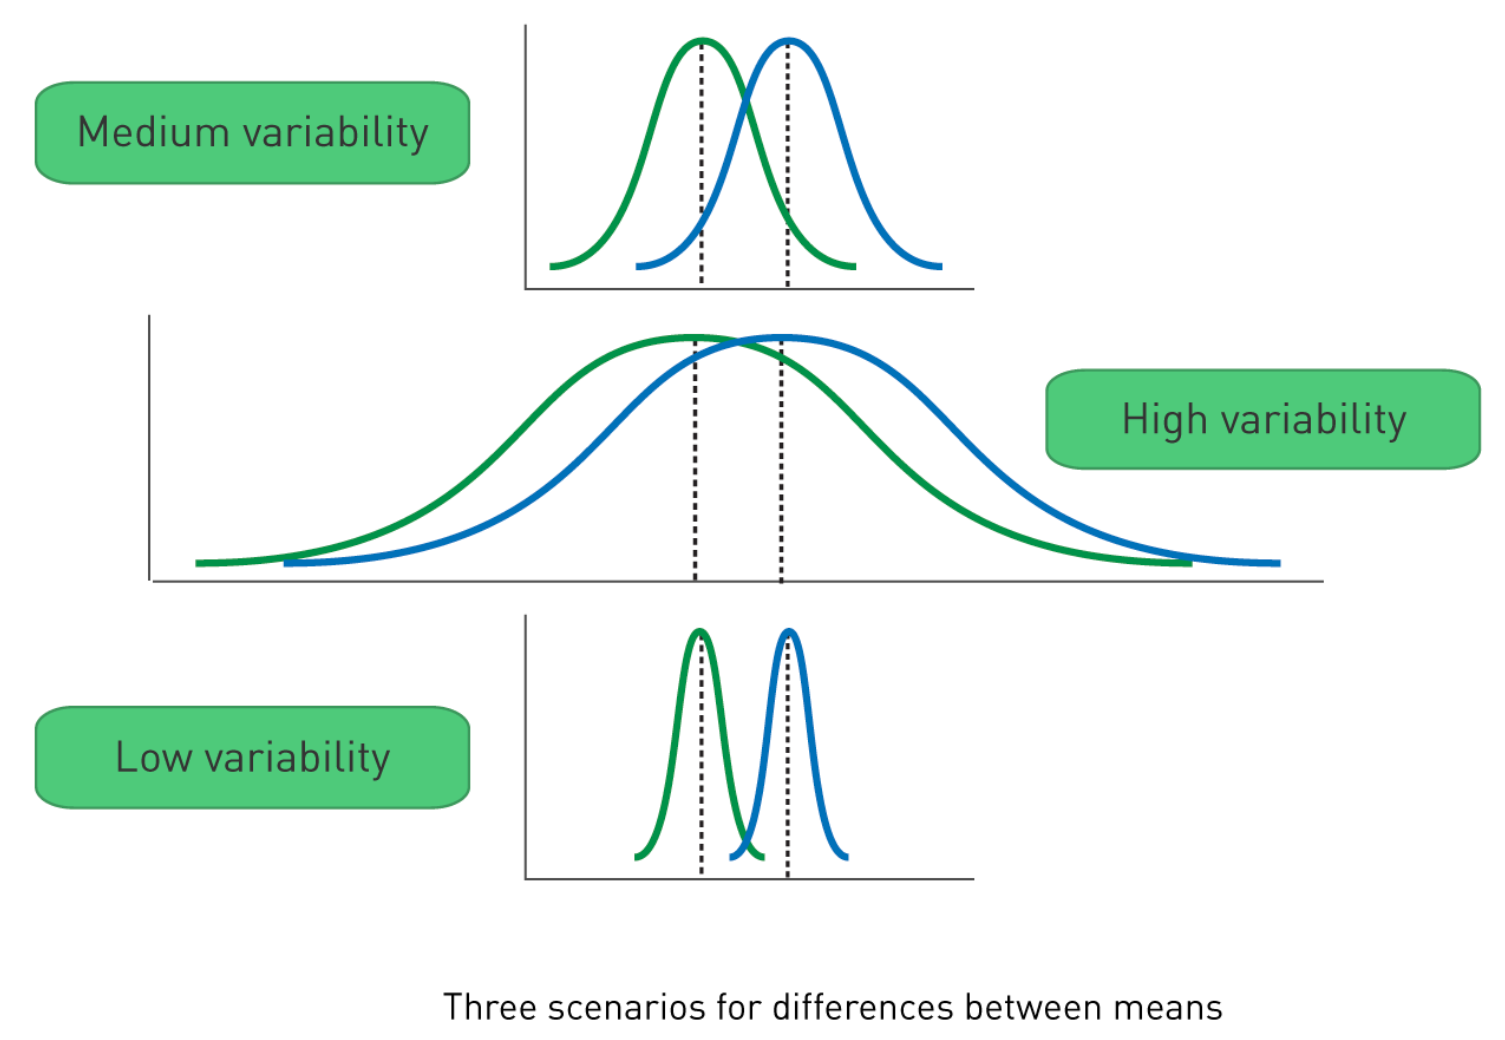
\includegraphics[width = 0.9\linewidth]{figures/t_test_scenarios.png}
    \end{center}
\end{frame}

\begin{frame}
  \frametitle{Comparing Population Means}
  \begin{exampleblock}{t-Test}
    Tells us whether the means of two sample populations are significantly different from each other 
    
    Allows us to test mean differences \textbf{while accounting for variability}
  \end{exampleblock}


\end{frame}


%Section 7.06 Edits end


%Section 7.08 Edits start

\section{Calculation of \textit{t}, Assumptions and Interpretations}

\begin{frame}
  \frametitle{\textit{t}-Test: Null and Alternative Hypotheses}

  \begin{exampleblock}{Null Hypothesis}
    $H_{0}: \mu_{1} = \mu_{c}$ (The two groups' means are equal)
  \end{exampleblock}
  
  \begin{exampleblock}{Alternative hypotheses}
    $H_{1}: \mu_{1} < \mu_{c}$ (group 1's mean is less than the other) \\
    $H_{2}: \mu_{1} > \mu_{c}$ (group 1's mean is greater than the other) \\
    $H_{3}: \mu_{1} \neq \mu_{c}$ (The two groups means not are equal)
  \end{exampleblock}
  \begin{itemize}
      \item $H_{3}$ is a \textbf{two-tailed} test
      \item $H_{1}$ and $H_{2}$ are \textbf{one-tailed} tests
  \end{itemize}
\end{frame}

\begin{frame}
  \frametitle{One- and Two-Tailed Tests: Defining Critical Regions}
  
  Three steps:
  \begin{enumerate}
      \item Form hypothesis
      \item Calculate $t$ statistic
      \item Plot $t$ value on the appropriate curve to get the $p$ value
  \end{enumerate}
\end{frame}

\begin{frame}
  \frametitle{The Independent Sample t-Test}

  $$t = \frac{\mu_{1}-\mu_{2}}{S_{\mu_{1}-\mu_{2}}} $$

  $$
    S_{\mu_{1}-\mu_{2}} = \sqrt{ (\frac{ (N_{1}-1)S_{1}^{2} + (N_{2}-1)S_{2}^{2} }{ N_{1}+N_{2}-2 })
                    (\frac{1}{ N_{1} } + \frac{1}{ N_{2} })
                  }
  $$

  $$
    t = \frac{(mean\ of\ group\ 1) - (mean\ of\ group\ 2)}{standard\ error\ of\ difference\ between\ means}
  $$
  
  
  \begin{exampleblock}{\textit{t} value}
    \textbf{Difference between group means} (mean difference), divided by the \textbf{variability of the two groups} (standard error of the differences)
  \end{exampleblock}

\end{frame}


\begin{frame}
  \frametitle{Degrees of Freedom}
  
  \begin{exampleblock}{degrees of freedom \textit{(df)}}
    Number of independent pieces of information that are allowed to vary
  \end{exampleblock}
  
  \begin{itemize}
    \item \textbf{Independent sample t-test}
    \begin{itemize}
      \item Uses two known quantities (the two group means)
      \item \textit{df} = $n_{1} + n_{2} -2$
    \end{itemize}
    \item \textbf{One sample t-test}
    \begin{itemize}
      \item \textit{df} = $n - 1$ (only uses one known quantity)
      \item Tests whether one sample's mean is significantly different from some hypothesized mean
    \end{itemize}
  \end{itemize}

\end{frame}
%Section 7.08 Edits end




\section{Practical Significance of the T-Test}
\begin{frame}
  \frametitle{Practical Significance for the T-Test}

  After using a t-test to assess statistical significance, it is
  important to assess practical significance. \\ \vspace{1em}

  \begin{quote}
    Your main goal is to explain to your audience
    why they should or should not care about the effect.
  \end{quote}

  \textbf{Three common effect size measures:}

  \begin{enumerate}
  \item Difference in means
  \item Cohen's d
  \item Correlation r
  \end{enumerate}
\end{frame}

\begin{frame}
  \frametitle{Difference in Means}

  \begin{block}{Difference in means}
    \[
      \bar{X}_{A} - \bar{X}_{B}
    \]
  \end{block}
    \begin{itemize}
    \item Answers the question ``\textit{How different are these
        groups?''}
    \item Often makes great headlines
      and is a good choice if units are familiar
    \item But lacks context in its calculation
  \item People who eat chocolate live 1.5 years longer than those who
    do not each chocolate
  \end{itemize}
\end{frame}


  \begin{frame}
    \frametitle{Cohen's d}

    \begin{block}{Cohen's d}
      \small
    \textit{Cohen's d} is a measure of difference of means
    standardized by the variance in the data.
    \[
      \frac{ \bar{X}_{A} - \bar{X}_{B} }{s}
    \]
    Where $s$ is a pooled standard deviation:
    $\sqrt \frac{(n_1-1)s_1^2 + (n_2-1)s_2^2}{n_1+n_2}$
  \end{block}

  \begin{itemize}
  \item Answers the question ``\textit{How many standard
      deviations apart are the groups?}''
  \item The difference in sarcasm score between frequentists and
    Bayesians is $d = 0.54$ standard deviations.
  \end{itemize}
\end{frame}

\begin{frame}
  \frametitle{Correlation}
  \note[item]{Notice the similarity in the form between Cohen's d and
    correlation -- Cohen's d divides by the pooled standard deviation;
    correlation divides by the product of two group standard
    deviations.}
  \begin{block}{Correlation}
    \textit{Correlation} answers the question ``How strong is the
    relationship between group identity and the outcome?''
    \[
      \rho = \frac{\cov(X, Y)}{\sigma_{X}\sigma_{Y}}
    \]
  \end{block}

  \begin{center}
    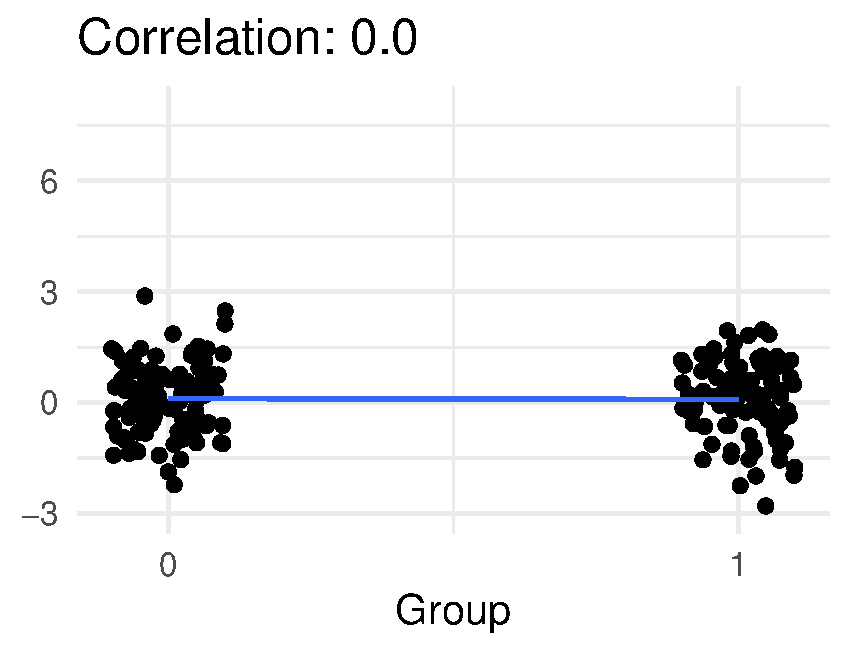
\includegraphics[width = 0.5\linewidth]{./figures/biserial_00}
  \end{center}
\end{frame}

\begin{frame}
  \frametitle{Correlation}

  \begin{block}{Biserial correlation}
    \textit{Correlation} answers the question ``How strong
    is the relationship between group identity and the outcome?''
    \[
      \rho = \frac{\cov(X, Y)}{\sigma_{X}\sigma_{Y}}
    \]
  \end{block}

  \begin{center}
    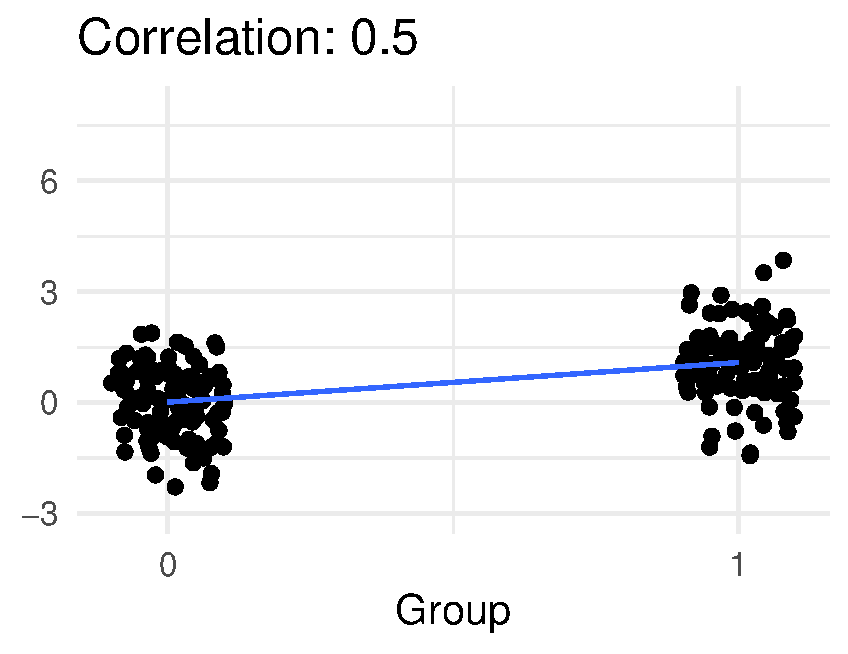
\includegraphics[width = 0.4\linewidth]{./figures/biserial_05}
  \end{center}
\end{frame}

\begin{frame}
  \frametitle{Correlation}

  \begin{block}{Biserial correlation}
    \textit{Correlation} answers the question ``How strong
    is the relationship between group identity and the outcome?''
    \[
      \rho = \frac{\cov(X, Y)}{\sigma_{X}\sigma_{Y}}
    \]
  \end{block}

  \begin{center}
    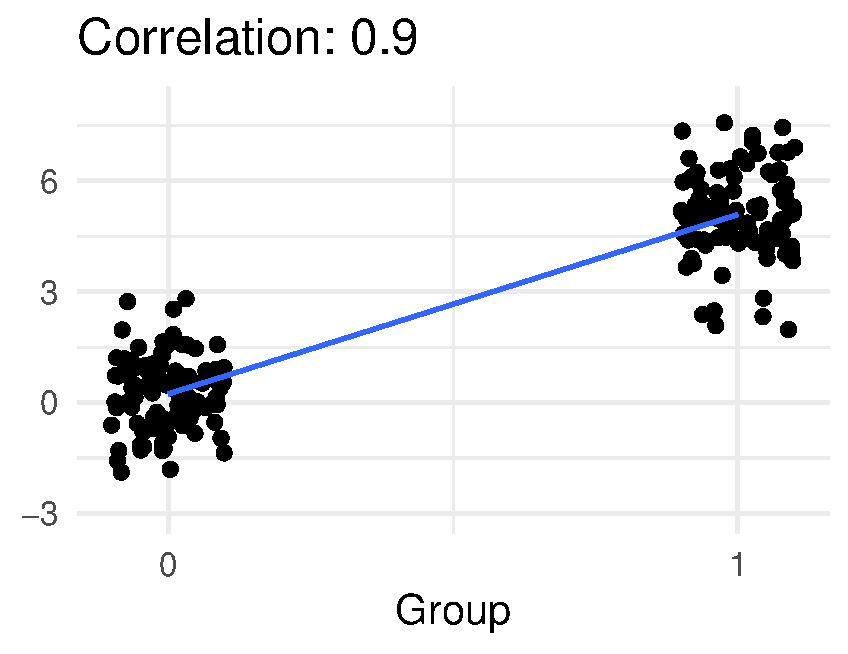
\includegraphics[width = 0.4\linewidth]{./figures/biserial_09}
  \end{center}
\end{frame}

\begin{frame}
  \frametitle{Practical Significance is about Context}

  \begin{itemize}
  \item How strong is the same relationship between \textit{different}
    groups?
  \item How strong is a \textit{different} relationship between the
    same group?
  \item What is the underlying dispersion in the data?
  \item What is a meaningful anchor or reference point that you can
    use for context?
  \end{itemize}
\end{frame}

\section{The Paired t-Test}

\begin{frame}
  \frametitle{Paired t-Test}

  \begin{exampleblock}{Climbing grip}
    Suppose you randomly sample 30 Berkeley students.  For each
    student $i$, you measure right-hand strength ($R_i$) and left-hand
    strength ($L_i$).

    \begin{itemize}
    \item You conduct a t-test with $H_0: \E[R] = \E[L]$
    \item \textbf{Problem}: Grip strength varies a lot
      person-to-person, $\Rightarrow$  t-test has low power.
    \end{itemize}
  \end{exampleblock}
\end{frame}

\begin{frame}
  \frametitle{Paired t-test}
  \centering
  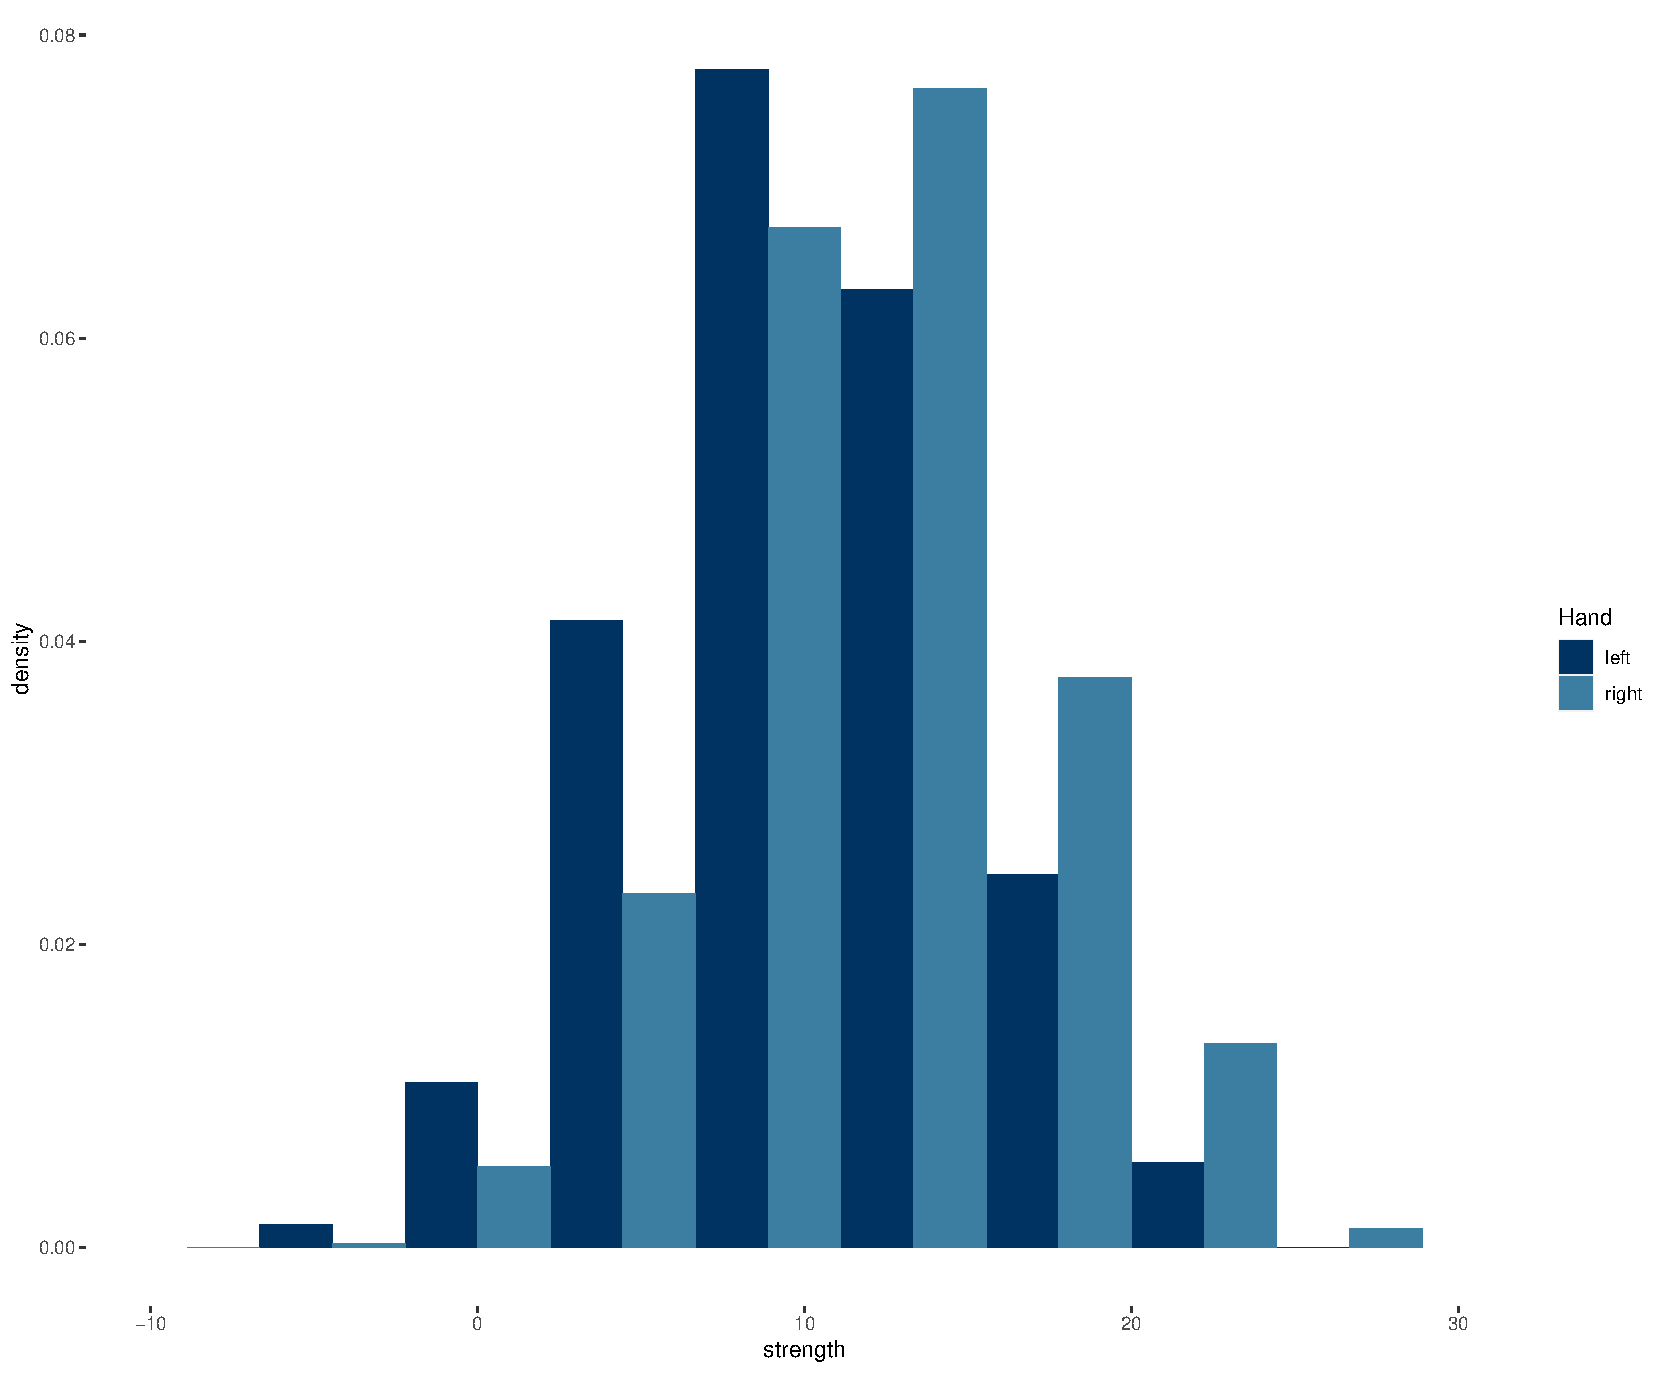
\includegraphics[width=.9\linewidth]{./figures/histogram_unpaired.pdf}
\end{frame}

\begin{frame}
  \frametitle{Paired t-Test}

  \begin{itemize}
  \item \textbf{Idea:} For any \textit{particular} subject $i$, the difference
    between right-hand strength and left-hand stregth, $R_i - L_i$,
    will usually be small.
  \item Within-person variation is small.
  \end{itemize}

  \begin{center}
    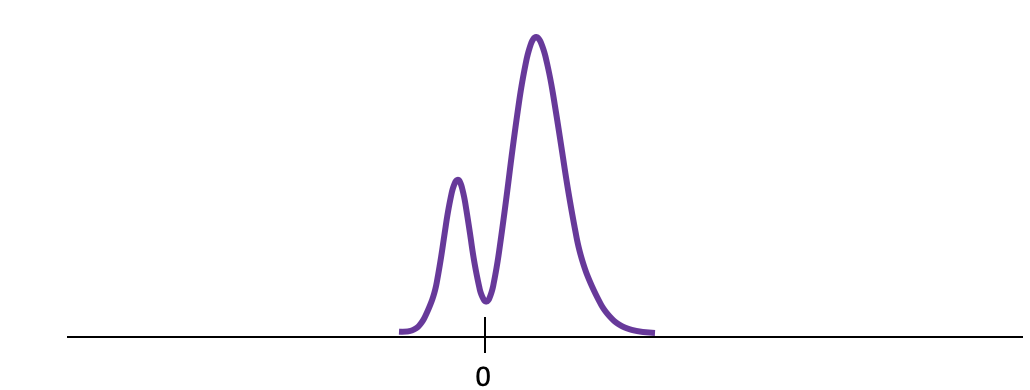
\includegraphics[width=.9\linewidth]{./figures/grip}
  \end{center}
\end{frame}

\begin{frame}
  \frametitle{Paired t-Test}
  \centering
    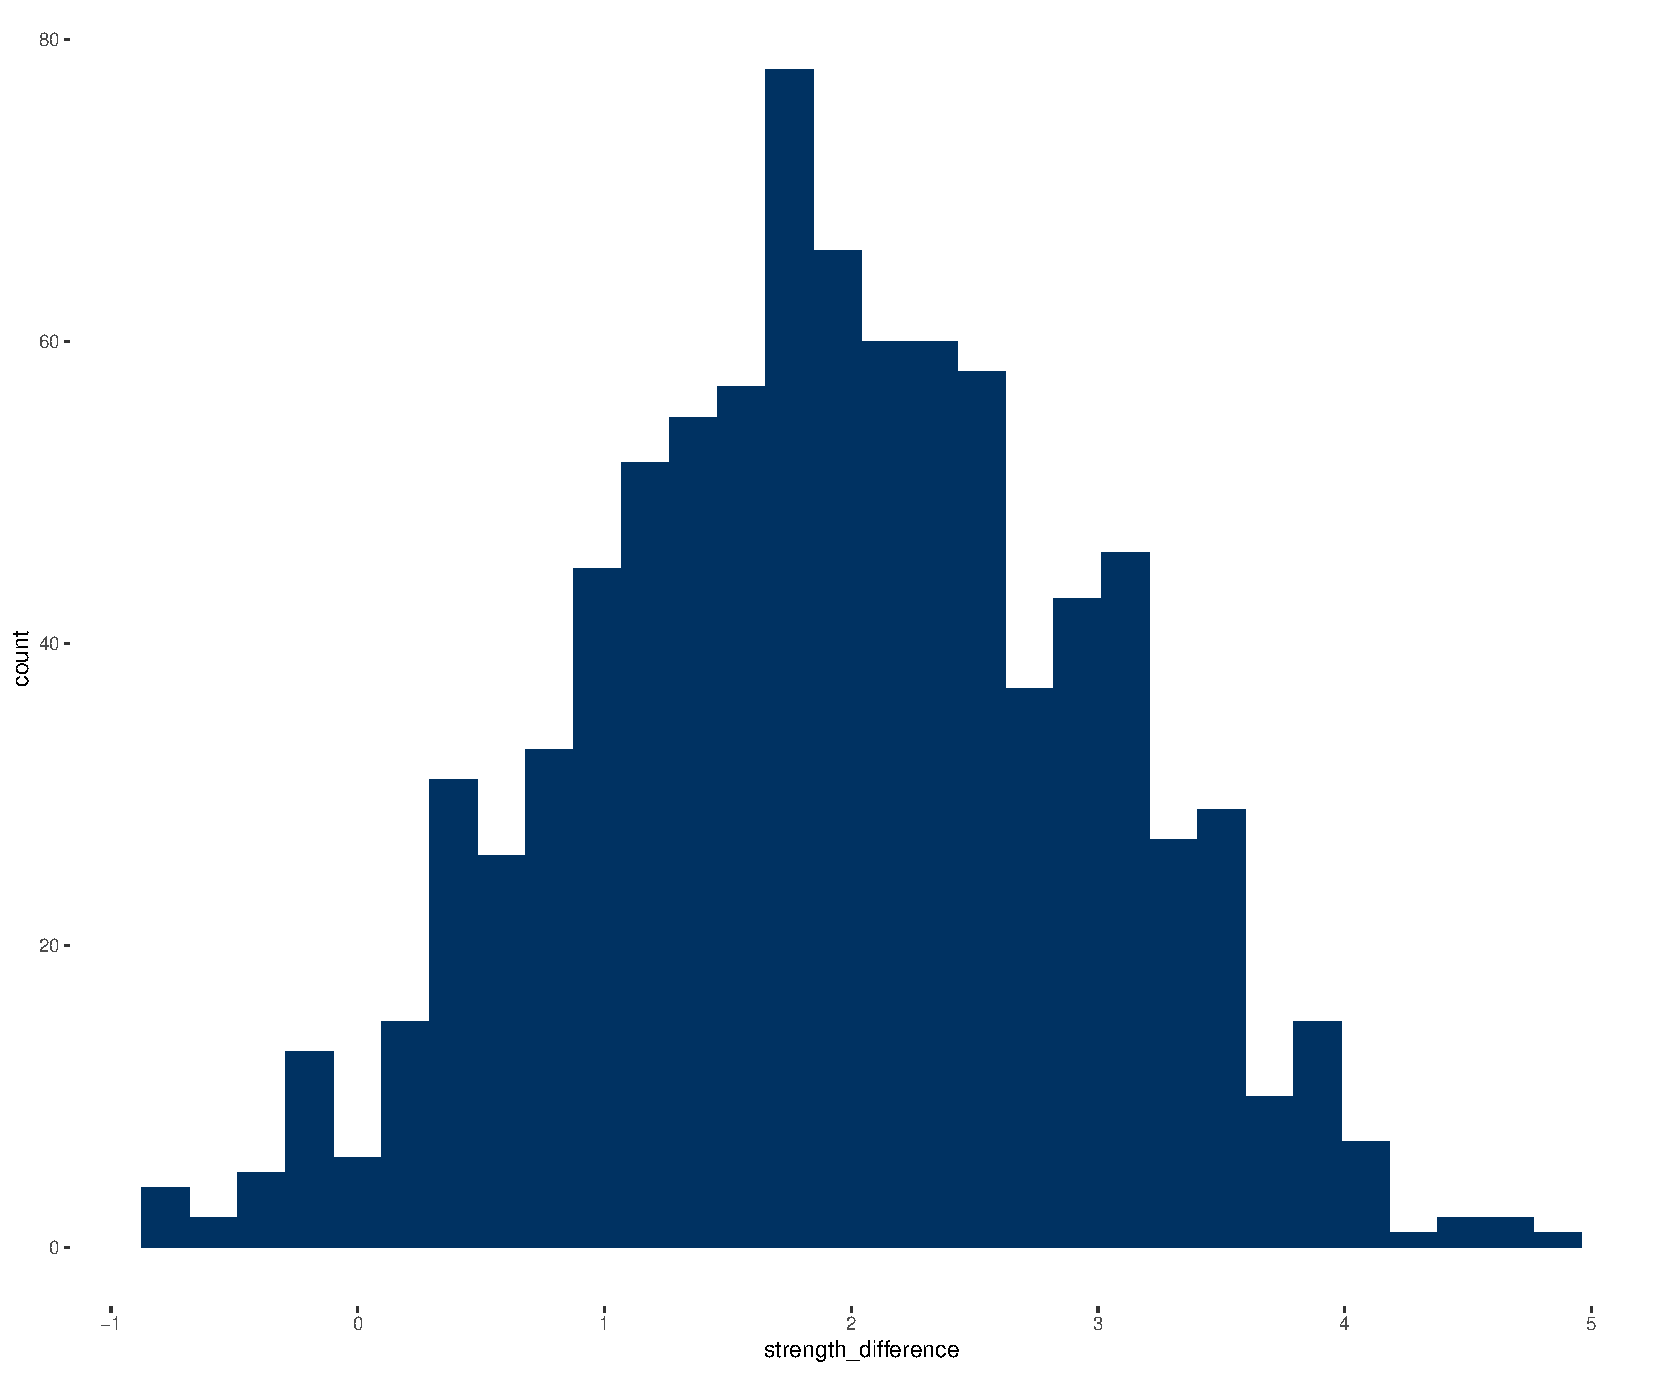
\includegraphics[width=.9\linewidth]{./figures/histogram_paired.pdf}
\end{frame}

\begin{frame}
  \frametitle{Paired t-Test}
  \centering
    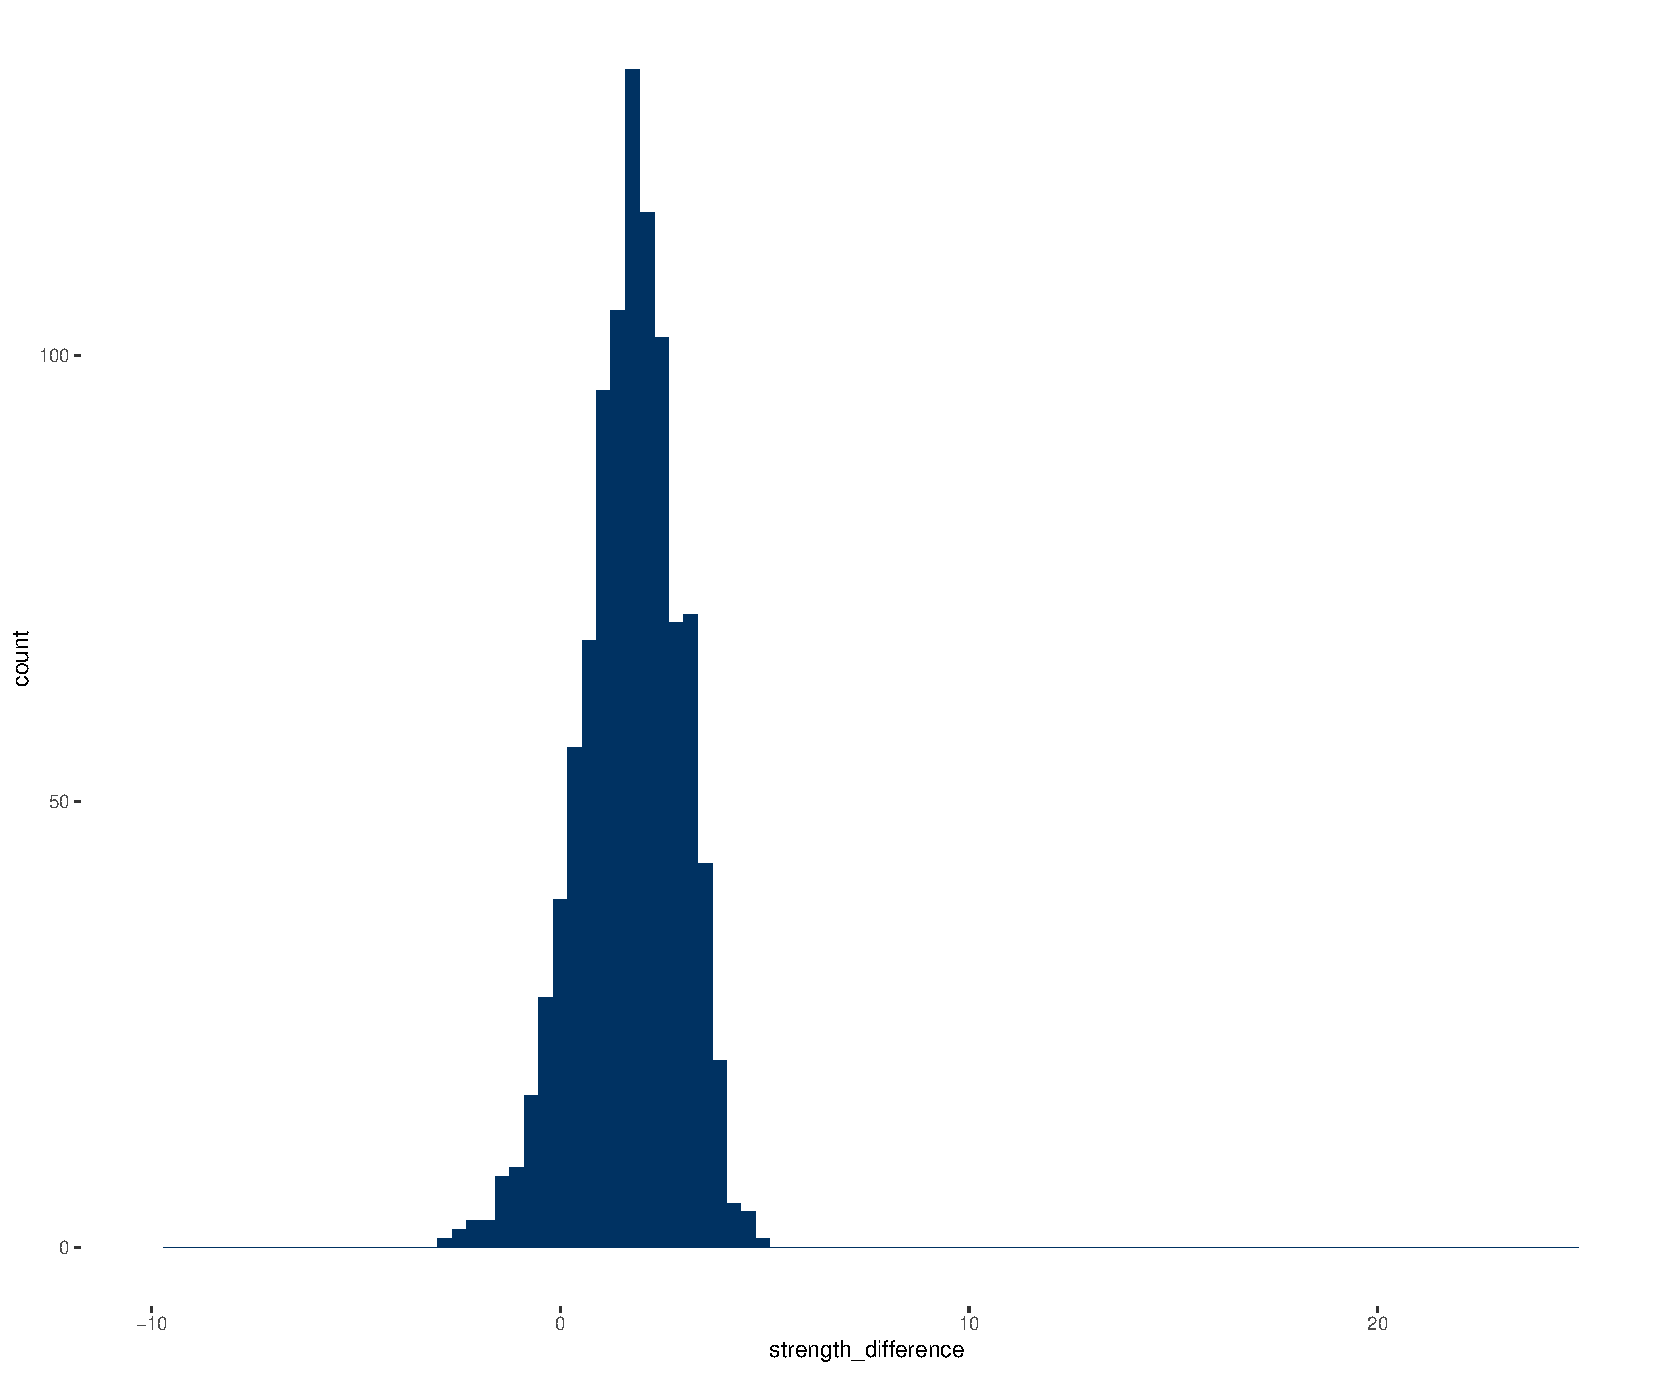
\includegraphics[width=.9\linewidth]{./figures/histogram_paired_rescaled.pdf}
\end{frame}

\begin{frame}
  \frametitle{Paired t-Test}
  \begin{block}{Paired t-test}
    A \textit{paired t-test}, sometimes called a \textit{dependent
      t-test}, builds an explicit dependency between data.
    Instead, perform a one-sample t-test with $H_0: \E[ R_{i}- L_{i}] = 0$.
  \end{block}
  \begin{itemize}
  \item This dependency must actually exist
  \item Cannot simply change the test
  \end{itemize}
\end{frame}

\begin{frame}
  \frametitle{Unpaired vs. Paired t-Test}

  \begin{columns}[t]
    \column{.49\linewidth}
    \textbf{Unpaired}
    \begin{itemize}
      \item $t = \frac{\bar{A} - \bar{B}} {\sigma_{A\&B}}$
    \end{itemize}
    \column{.49\linewidth}
    \textbf{Paired}
    \begin{itemize}
    \item $t = \frac{\bar{A} - \bar{B}}{\sigma_{(A - B)}}$
    \end{itemize}
  \end{columns}

\end{frame}

\begin{frame}
  \frametitle{Paired t-Test Assumptions}

  \begin{itemize}
  \item $A$ and $B$ have a metric scale with the same units.
  \item There is a natural pairing between observations for $A$ and for $B$.
    \begin{itemize}
    \item pre-test and post-test for same individual
    \item response to two types of stimulus for same mouse
    \item responses for a pair of spouses
    \end{itemize}
  \item Each pair $(A_i, B_i)$ is drawn i.i.d.
  \item The distribution of $A-B$ is sufficiently normal given the sample size.

  \end{itemize}
\end{frame}



%Start section 7.17 edits
\section{Introduction to Non-parametric Tests}

\begin{frame}
  \frametitle{Non-parametric Tests}
  
  \begin{itemize}
    \item $t$-test is parametric, like all the tests we've seen so far
    \begin{itemize}
      \item Assumes the population comes from a parametric family of distributions
      \item Typically the normal curves
    \end{itemize}
    \item It is not always possible to meet this assumption
  \end{itemize}
  
\end{frame}


\begin{frame}
  \frametitle{Non-parametric Tests (cont.)}    

  \textbf{Large sample} 
  \begin{itemize}
    \item No Problem
    \item central limit theorem tells us that the sampling distribution of the mean will be approximately normal, so $t$-tests are valid
    \item Parametric tests are generally valid for large samples
  \end{itemize}

\end{frame}


\begin{frame}
  \frametitle{Non-parametric Tests (cont.)}
  
  \textbf{Small sample}
  \begin{itemize}
    \item $t$-test is fairly robust to deviations from normality, but you should look at your distribution and see how non-normal it is
    \item Suppose you have a small sample and you suspect you have a major deviation from normality
    \item You might be able to transform the variable to make it more normal, but that can alter the meaning and make results harder to interpret
  \end{itemize}
  
  
  \begin{exampleblock}{An alternative is to use a \textit{non-parametric} test}
    
  \end{exampleblock}
  
    
\end{frame}

\begin{frame}
  \frametitle{Non-parametric Test Details}
  
  \begin{itemize}
      \item Non-parametric tests can be also called \textbf{distribution- free tests}
      \begin{itemize}
          \item Still involve assumptions, but they are less restrictive than those of parametric tests
      \end{itemize}
      \item Many tests work on principle of ranking data
      \begin{itemize}
          \item List the scores from lowest to highest -- each score gets a rank, so higher scores have higher ranks
          \item Only consider ranks instead of looking at the metric value of the variable
          \item Use the order of variables to construct statistics that we can use to test hypotheses
      \end{itemize}
  \end{itemize}
    
\end{frame}


\begin{frame}
  \frametitle{Non-parametric Test Details (cont.)}
  \begin{columns}
    \column{0.5\textwidth}
    \textbf{Advantages}
    \begin{itemize}
        \item Population distribution doesn't have to be normal
        \item Easier to justify a rank-based test
    \end{itemize}
    
    \column{0.5\textwidth}
    \textbf{Disadvantages}
    \begin{itemize}
        \item We throw out metric information
        \item Rule of thumb: if you throw away information, you lose statistical pwoer
    \end{itemize}
  \end{columns}
    
\end{frame}


\begin{frame}
  \frametitle{Rank-Based Tests for Ordinal Variables}
  \begin{itemize}
      \item Rank-based tests are especially useful when we have an ordinal variable 
      \begin{itemize}
          \item eg. a Likert variable such as "how do you feel about a presidential campaign?"
          \item Neutral, support, strongly support, etc.
      \end{itemize} 
      \item It is hard to argue that the difference between neutral and support is the same as the difference between support and strongly support
  \end{itemize}
    
\end{frame}


\begin{frame}
  \frametitle{Love Tester Example}
  
  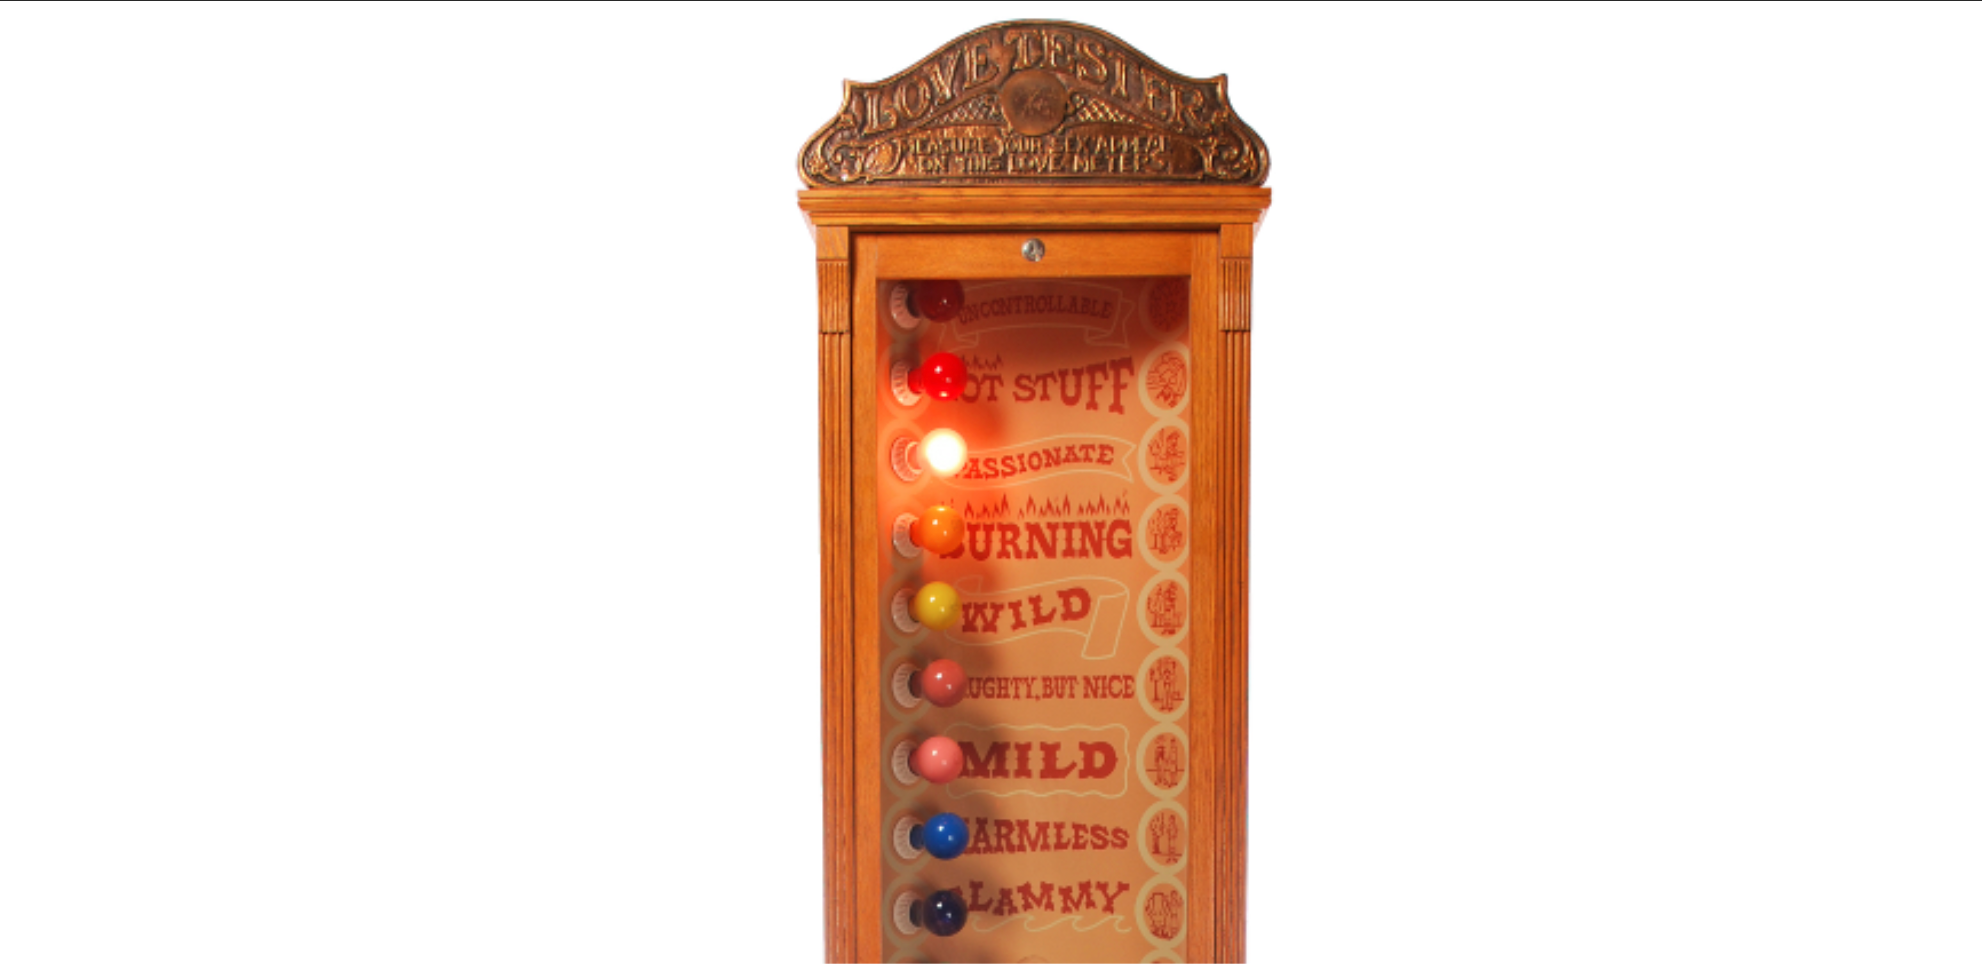
\includegraphics[width=1.0\textwidth]{figures/love_tester.png}

  Do you trust that the difference between harmless and mild is the same as the difference between burning and passionate?
    
\end{frame}

\begin{frame}
  \frametitle{Rank-Based Tests for Ordinal Variables (cont.)}
  
  If you run a $t$-test in these cases, you impose a linear structure on your variable, treating it as metric
  \begin{itemize}
      \item This method may or may not be reasonable
      \item If you use a rank-based test that is okay--you are asking whether one group tends to rank below or above another 
      \item The ranks are still meaningful
  \end{itemize}
    
\end{frame}


\begin{frame}
  \frametitle{Conclusion}

  \begin{itemize}
    \item There are some situations in which you should consider non-parametric tests
    \item Coye is going to tell you more about the specifics
  \end{itemize}
  
\end{frame}




%End section 7.17 edits







%Start section 7.19 edits
\section{Wilcoxon Rank-sum Test for Independent Groups}


\begin{frame}
  \frametitle{Parametric and Non-parametric Tests for Comparing Only Two Groups}

  \begin{center}
    \begin{tabular}{p{0.3\linewidth}||p{0.3\linewidth}|p{0.3\linewidth}}
      \textbf{Type of Design} & \textbf{Parametric Tests} & \textbf{Non-parametric Tests}  \\
      \hline \hline
      \textit{Two independent samples}  & Independent samples $t$ test & Wilcoxon rank-sum test (Mann-Whitney test) \\
      \hline
      \textit{Two dependent Samples } & Dependent samples $t$ test & Wilcoxon signed-rank test
    \end{tabular}   
  \end{center}

\end{frame}


\begin{frame}
  \frametitle{Comparing Two Independent Conditions: Wilcoxon Rank-Sum Test}
  
  \begin{itemize}
    \item Data are ranked from lowest to highest across groups
    \item This provides \textbf{potential rank} scores
    \item If the same score occurs more than once then all scores of the same value receive the average of the potential ranks for those scores
  \end{itemize}
  
  \begin{center}
    \scalebox{0.4}{  
      \begin{tabular}{c|cccc}
        ID & Group & Score & Potential Rank & Final Rank \\ \hline
        1  & A     & 10    & 1              & 1   \\ 
        2  & A     & 11    & 2              & 2.5 \\ 
        3  & B     & 11    & 3              & 2.5 \\ 
        4  & B     & 12    & 4              & 4   \\ 
        5  & A     & 20    & 5              & 6   \\
        6  & B     & 20    & 6              & 6   \\
        7  & B     & 20    & 7              & 6   \\
        8  & A     & 33    & 8              & 8   \\
      \end{tabular}
    }
  \end{center}

  \begin{itemize}
      \item This gives us the \textbf{final rank} scores
  \end{itemize}
\end{frame}


\begin{frame}
  \frametitle{Comparing Two Independent Conditions: Wilcoxon Rank-Sum Test}

  \begin{center}
    \begin{tabular}{c|cccc}
      ID & Group & Score & Potential Rank & Final Rank \\ \hline
      1  & A     & 10    & 1              & 1   \\ 
      2  & A     & 11    & 2              & 2.5 \\ 
      3  & B     & 11    & 3              & 2.5 \\ 
      4  & B     & 12    & 4              & 4   \\ 
      5  & A     & 20    & 5              & 6   \\ 
      6  & B     & 20    & 6              & 6   \\ 
      7  & B     & 20    & 7              & 6   \\ 
      8  & A     & 33    & 8              & 8   \\
    \end{tabular}
  \end{center}

\end{frame}


\begin{frame}
  \frametitle{Calculating the Wilcoxon Rand-Sum Test}
  
  \begin{itemize}
    \item After assigning final ranks, add up all the final ranks for each of the two groups
    \item Subtract the mean rank for a group of the same size as our groups
    \begin{itemize}
      \item Otherwise, larger groups would always have larger values
      \item For example, the mean group for a group of four = 1 + 2 + 3 + 4 = 10
    \end{itemize}
    \item Our final calculation in therefore:
    \begin{itemize}
      \item $W$ = sum of ranks - mean rank
    \end{itemize}
  \end{itemize}
    
\end{frame}


\begin{frame}
  \frametitle{Calculating the Wilcoxon Rank-Sum Test (cont.)}
  
  \begin{center}
    \scalebox{0.75}{  
      \begin{tabular}{c|cccc}
        ID & Group & Score & Potential Rank & Final Rank \\ \hline
        1  & A     & 10    & 1              & 1   \\
        2  & A     & 11    & 2              & 2.5 \\ 
        3  & B     & 11    & 3              & 2.5 \\ 
        4  & B     & 12    & 4              & 4   \\ 
        5  & A     & 20    & 5              & 6   \\
        6  & B     & 20    & 6              & 6   \\
        7  & B     & 20    & 7              & 6   \\
        8  & A     & 33    & 8              & 8   \\
      \end{tabular}
    }
  \end{center}

  \begin{itemize}
    \item Group A: W = sum of ranks (17.5) - mean rank (10) = 7.5
  \end{itemize}
    
\end{frame}


\begin{frame}
  \frametitle{Interpretation of the Wilcoxon Rank-Sum Test}

  \begin{exampleblock}{Default is a two-sided test, like a \textit{t} test}
    \textbf{Null hypothesis:} There is no difference in ranks
    \textbf{Alternative hypothesis:} There is a difference in ranks
  \end{exampleblock}
  
  \begin{itemize}
      \item You can also do a one-directional test if you hypothesize that one particular group will have higher ranks than the other
      \item Always two values for $W$ (one for each group)
      \item Lowest score for $W$ is typically used as the test statistic
  \end{itemize}
  
\end{frame}

\begin{frame}
  \frametitle{Interpretation of the Wilcoxon Rank-Sum Test (cont.)}
  
  \begin{itemize}
      \item For small sample sizes (N<40), R calculates the $p$ value with the Monte Carlo methods
      \begin{itemize}
          \item ie. simulated data are used to estimate the statistic
      \end{itemize}
      \item For larger samples, R calculates the $p$ value with a normal approximation method
      \begin{itemize}
          \item Assumes that the sampling distribution of the $W$ statistic is normal, not the data
          \item Normal approximation method helpful because it calculates a z statistic in the process of calculating the $p$ value
      \end{itemize}
  \end{itemize}
    
\end{frame}

\begin{frame}
  \frametitle{Effect Size for the Wilcoxon Rank-Sum Test}

  \begin{exampleblock}{Effect Size Correlation}
    $$r = \frac{Z}{ \sqrt{N} }$$
    Divide the z statistic by the square root of the total sample size
  \end{exampleblock}

  \begin{center}
  \begin{tabular}{c|c}
    r    & Effect Size  \\ \hline
    0.10 & Small \\
    0.30 & Medium \\
    0.50 & Large 
  \end{tabular}
  \end{center} 
\end{frame}

%End section 7.19 edits

\end{document}
